
\begin{figure}[htpb]

% This is first (1x1)
    \centering
    \begin{subfigure}[b]{0.47\textwidth}
     \centering
    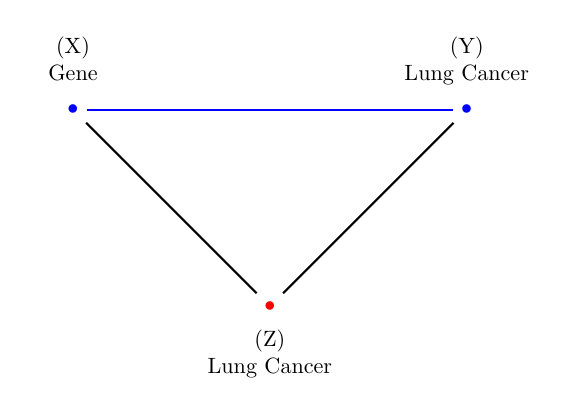
\begin{tikzpicture}[thick,scale=0.5, every node/.style={scale=0.8}]{
    \node [blue, label=above:\begin{tabular}{c}(Y)\\Lung Cancer\end{tabular}] (Y) at (10,10) {$\bullet$};
    \node [blue, label=above:\begin{tabular}{c}(X) \\Gene \end{tabular}] (X) at (0,10) {$\bullet$};
    \node [red, label=below:\begin{tabular}{c}(Z)\\Lung Cancer \end{tabular}] (Z) at (5,5) {$\bullet$};

    \path (X) edge (Z);
    \path [blue] (X) edge (Y);
    \path (Y) edge (Z);
    }
\end{tikzpicture}
    \caption{Regular Collider}
    \label{Regular_Collider}
    \end{subfigure}
\hfill
% This is second (1x2)
    \begin{subfigure}[b]{0.47\textwidth}
    \centering
        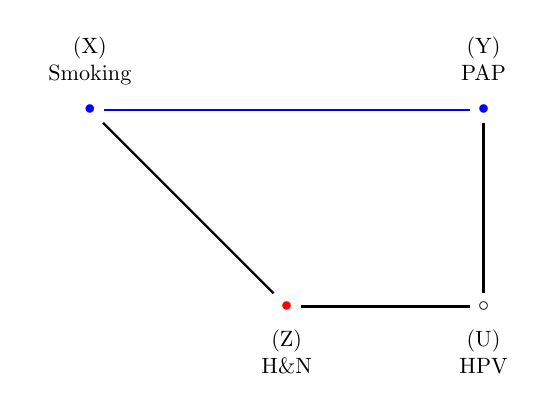
\begin{tikzpicture}[thick,scale=0.5, every node/.style={scale=0.8}]{
    \node [label=below:\begin{tabular}{c}(U)\\HPV\end{tabular}] (U) at (15,5) {$\circ$};
    \node [blue, label=above:\begin{tabular}{c}(X)\\Smoking\end{tabular}] (X) at (5,10) {$\bullet$};
    \node [red, label=below:\begin{tabular}{c}(Z)\\H\&N\end{tabular}] (Z) at (10,5) {$\bullet$};
    \node [blue, label=above:\begin{tabular}{c}(Y)\\PAP\end{tabular}] (Y) at (15,10) {$\bullet$};

    \path (U) edge (Z);
    \path (U) edge (Y);
    \path (X) edge (Z);
    \path [blue](X) edge (Y);
    }
\end{tikzpicture}
\caption{Forked Collider}
\label{Forked_Collider}

    \end{subfigure}\\



% This is third (2x1)
    \begin{subfigure}[b]{0.47\textwidth}
        \centering
    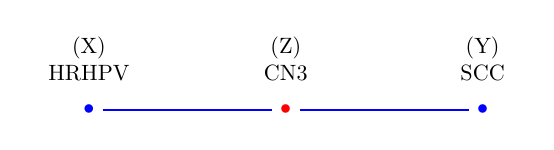
\begin{tikzpicture}[thick,scale=0.5, every node/.style={scale=0.8}]{
    
    \node [blue, label=above:\begin{tabular}{c}(Y)\\SCC\end{tabular}] (Y) at (10,5) {$\bullet$};
    \node [blue, label=above:\begin{tabular}{c}(X)\\HRHPV\end{tabular}] (X) at (0,5) {$\bullet$};
    \node [red, label=above:\begin{tabular}{c}(Z)\\CN3\end{tabular}] (Z) at (5,5) {$\bullet$};

    \path [blue] (X) edge (Z);
    \path [blue] (Z) edge (Y);
    }
\end{tikzpicture}
    \caption{Regular Pipe}
    \label{Regular_Pipe}

    \end{subfigure}
\hfill
% this is fourth (2x2)
    \begin{subfigure}[b]{0.47\textwidth}
         \centering
        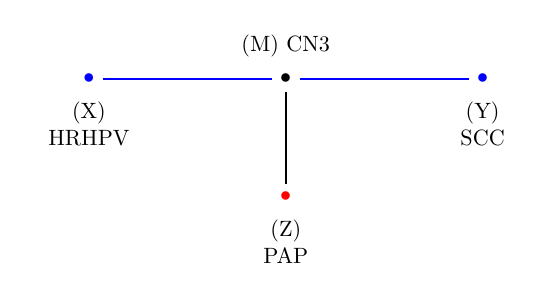
\begin{tikzpicture}[thick,scale=0.5, every node/.style={scale=0.8}]{
    \node [blue, label=below:\begin{tabular}{c}(Y)\\SCC\end{tabular}] (Y) at (10,3) {$\bullet$};
    \node [blue, label=below:\begin{tabular}{c}(X)\\HRHPV\end{tabular}] (X) at (0,3) {$\bullet$};
    \node [label=above:(M) CN3] (M) at (5,3) {$\bullet$};
    \node [red, label=below:\begin{tabular}{c}(Z)\\PAP\end{tabular}] (Z) at (5,0) {$\bullet$};
    \path [blue](X) edge (M);
    \path [blue] (M) edge (Y);
    \path (M) edge (Z);
    }
\end{tikzpicture}
    \caption{Pipe's Descendent}
    \label{Pipe_s_Decendent}
    \end{subfigure}\\

% this is fifth (3x1)
\begin{subfigure}[b]{0.47\textwidth}
         \centering
       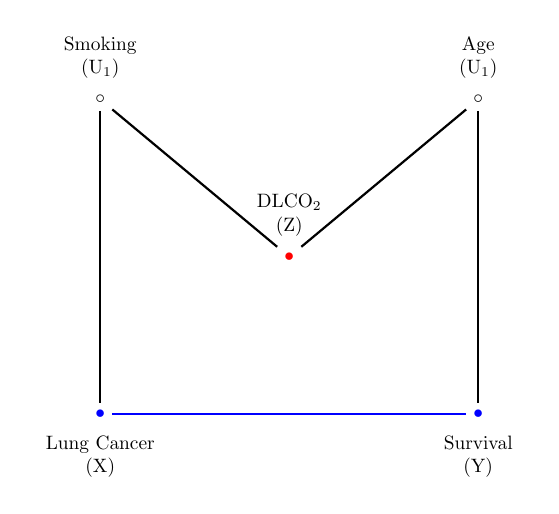
\begin{tikzpicture}[thick,scale=0.4, every node/.style={scale=0.7}]{
    \node [label=above:\begin{tabular}{c}Smoking\\(U\textsubscript{1})\end{tabular}] (Smoking) at (0,10) {$\circ$};
    \node [label=above:\begin{tabular}{c}Age\\(U\textsubscript{1})\end{tabular}] (Age) at (12,10) {$\circ$};
    \node [blue, label=below:\begin{tabular}{c}Lung Cancer\\(X)\end{tabular}] (LungCancer) at (0,0) {$\bullet$};
    \node [blue,label=below:\begin{tabular}{c}Survival\\(Y)\end{tabular}] (Survival) at (12,0) {$\bullet$};
    \node [red, label=above:\begin{tabular}{c}DLCO\textsubscript{2}\\(Z)\end{tabular}] (Measure) at (6,5) {$\bullet$};
    
    \path (Smoking) edge (LungCancer);
    \path (Age) edge (Survival);
    \path [blue](LungCancer) edge (Survival);
    \path (Smoking) edge (Measure);
    \path (Age) edge (Measure);
    }
\end{tikzpicture}
\caption{M-Bias}
    \label{M-Bias}
    \end{subfigure}
\hfill
    % this is sixth (3x2)
\begin{subfigure}[b]{0.47\textwidth}
         \centering
      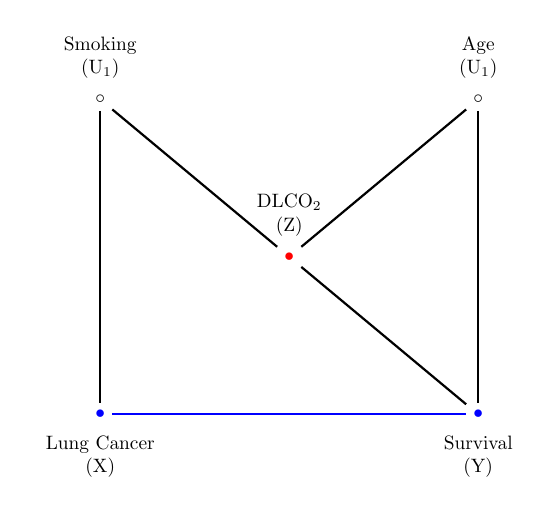
\begin{tikzpicture}[thick,scale=0.4, every node/.style={scale=0.7}]{
    \node [label=above:\begin{tabular}{c}Smoking\\(U\textsubscript{1})\end{tabular}] (Smoking) at (0,10) {$\circ$};
    \node [label=above:\begin{tabular}{c}Age\\(U\textsubscript{1})\end{tabular}] (Age) at (12,10) {$\circ$};
    \node [blue, label=below:\begin{tabular}{c}Lung Cancer\\(X)\end{tabular}] (LungCancer) at (0,0) {$\bullet$};
    \node [blue, label=below:\begin{tabular}{c}Survival\\(Y)\end{tabular}] (Survival) at (12,0) {$\bullet$};
    \node [red, label=above:\begin{tabular}{c}DLCO\textsubscript{2}\\(Z)\end{tabular}] (DLCO) at (6,5) {$\bullet$};
    
    \path (Smoking) edge (LungCancer);
    \path (Age) edge (Survival);
    \path [blue] (LungCancer) edge (Survival);
    \path (Smoking) edge (DLCO);
    \path (Age) edge (DLCO);
    \path (DLCO) edge (Survival);
}
\end{tikzpicture}
\caption{Undecidable Case }
    \label{Undecidable_Case}
    \end{subfigure}
 \caption{\textbf{Bad Controls}}
 \label{Bad_Controls}
\end{figure}